\documentclass[sigconf, anonymous, review]{acmart}
\usepackage{booktabs}
\usepackage{amsmath}
\usepackage{graphicx}
\usepackage{placeins}
\usepackage{xcolor}
\usepackage{multirow}
\usepackage{float}
\usepackage{subcaption}
\usepackage{enumitem}
\usepackage{tikz}
\usetikzlibrary{arrows.meta,positioning,fit,calc,backgrounds,decorations.pathreplacing}
\hypersetup{colorlinks=true,linkcolor=blue,citecolor=blue,urlcolor=blue}
\setlength{\emergencystretch}{1em}

\begin{document}

\title[ScrapeBench]{ScrapeBench: An Acquisition Contract for Face Consent on the Agentic Web}

\author{Anonymous Author(s)}
\affiliation{\institution{Anonymous Institution}\city{Anonymous}\country{Anonymous}}

\begin{abstract}
On a Web increasingly read by generative agents, publishing a face and consenting
to model customization have become technically indistinguishable. Existing
anti-customization methods are evaluated on pristine files, although an agent
may acquire a photograph after a single ordinary Web operation such as CDN
transcoding, thumbnail rendering, screenshot cropping, restoration,
regeneration, or purification. We introduce \emph{ScrapeBench}, an acquisition
contract that evaluates each such operation independently from the same upload,
with a matched clean branch and held-out identity references. Our feasibility
pilot fixes four identities, with four gallery and two reference images per
identity, before inspecting defense outcomes. Completed comparisons cover
clean, GAP-Diff, MetaCloak, GoodAC, and ARCP-Web under InstantID and IP-Adapter-FaceID.
ARCP-Web allocates a bounded perturbation by texture and explicitly
optimizes the currently weakest of seven independent acquisition conditions.
We report conditional and end-to-end identity similarity, face-detection
failure, image quality, and paired identity-bootstrap intervals. Among 11
reader--layer conditions passing the clean validity gate, ARCP-Web obtains the
largest paired protection gap in nine, while respecting an 8/255 pixel budget
and attaining 37.80 dB PSNR. The small pilot is an effect-direction and systems
check, not a population estimate; a pre-audited 40-identity pool is used only
after its gates pass.

\end{abstract}

\ccsdesc[500]{Information systems~World Wide Web}
\ccsdesc[500]{Security and privacy~Privacy-preserving protocols}
\ccsdesc[300]{Computing methodologies~Computer vision}
\keywords{agentic web, face consent, anti-customization, web acquisition, evaluation contract}

\maketitle

\section{Introduction}

The web has become the default training corpus for identity-hungry generative models, and faces are its most sensitive commodity. A handful of public portraits suffices to synthesize a person in any context: DreamBooth-style fine-tuning binds a rare token to an identity with four to eight images~\cite{ruiz2022dreambooth}, while zero-shot adapters such as InstantID and IP-Adapter-FaceID inject a face embedding from a single reference image directly into the denoising process~\cite{wang2024instantid,ye2023ipadapter}. The consent asymmetry is severe---the subject never agreed---and it has triggered an arms race in \emph{protective perturbation}: cloaks added to a photo before upload that break the customization pipeline. Anti-DreamBooth established the category~\cite{le2023antidreambooth}, and a fast-growing successor literature hardens it along every laboratory axis~\cite{liu2023metacloak,zheng2023targeted,onikubo2024highfrequency,li2024promptindependent,song2024idprotector}. The narrative is reassuring: with the right perturbation, your face is yours again.

\textbf{Relevance to the Web.} Every component of this study is Web infrastructure: the protection gap is created and erased by platform image pipelines (CDNs, avatar services, thumbnailers), browser rendering, and crawling agents; the adversary is any scraper harvesting faces the way the Web serves them; and the proposed remedy is a machine-readable consent manifest served over the Web's ingestion layer. The paper answers a Responsible Web research challenge---measuring, then repairing, the distance between the privacy users believe they control and the acquisition pipeline the Web actually executes.

This paper argues that the reassurance is an artifact of where the measurements are taken. Every published protection is evaluated on \emph{T0-images}: clean, full-resolution, uncompressed files that the adversary kindly provides to the defense. That world does not exist on the web. An identity that is ``public'' has already been transformed before a scraper ever sees it: platforms re-encode uploads under storage and bandwidth budgets, browsers rasterize images under device pixel ratios and thumbnail pipelines, crawling agents screenshot pages and crop detected faces rather than download files, and users regenerate their photos through diffusion filters before posting. Each transformation is individually harmless to recognition; jointly, they describe the actual data distribution any real adversary can harvest. We call this pipeline the \emph{web acquisition funnel} and the resulting blind spot the \emph{Web Acquisition Gap}: the difference between the protection a defense delivers on the files it was handed and the protection that survives on the files an adversary can actually obtain---an attack surface that requires no adversarial optimization, costs milliseconds to seconds per image, and operates \emph{before} the defense is ever consulted.

Two observations sharpen the claim. First, the funnel is not hypothetical: a single JPEG re-encode at quality 85--95 neutralizes a broad class of protection perturbations~\cite{sandovalsegura2023jpeg}, common image transformations systematically suppress unlearnable-example attacks~\cite{qin2023learning,sandovalsegura2023what}, and robustness under diffusion-aware adversaries remains unfavorable~\cite{peng2025contrastive}. Nor is the funnel's parameter range speculative: our probes of production image pipelines (Section~\ref{sec:reality}) land squarely inside the transcode tiers we evaluate. What is missing is a systematic, tiered, budget-aware account of the entire funnel under both tunable and zero-shot attack pipelines. Meanwhile evaluation practice drifts the other way: newest defenses arrive with ever-cleaner galleries under ever-stronger laboratory attackers~\cite{fardin2026metacloakjpeg,chen2025fragile}, and the first cross-method studies still hold the acquisition side fixed~\cite{wang2025privacy}---a literature optimizing for an adversary that does not exist.

We build the missing instrument. \emph{ScrapeBench} reconstructs the funnel in software: seven tiers (T0 original; T1 platform transcode; T2 browser and thumbnail rendering; T3 agent-style capture; T4 super-resolution; T5 diffusion regeneration; T6 adaptive mixing and purification), each with an explicit attacker budget. On top of it we define the \emph{retention ratio} $\mathrm{RR}(T)=\Delta(T)/\Delta(T_0)$, where $\Delta(T)$ is the protection gap (clean minus protected identity similarity under a fixed attack) at tier $T$: RR is the fraction of a defense's T0 gap that survives acquisition reality, computed against a same-identity clean control. The primary evaluation applies each of six representative preprocessing operations (JPEG-85, WebP-80, browser render, agent face-crop, super-resolution, diffusion regeneration) \emph{in isolation}, because the marginal damage a single operation does to a protection gap is the quantity a defender can act on; stacking operations multiplies combinatorics faster than it multiplies insight, and a completed composition study (Appendix~\ref{sec:extra}) confirms that reordering or deepening the chain does not rescue a gap. The metric is paired with a cost ledger: the defender pays GPU-minutes per identity to forge a perturbation, the attacker pays CPU-milliseconds per image to defeat it.

Running ScrapeBench over 40 public identities, two published defenses (FSMG-style untargeted surrogate attacks~\cite{le2023antidreambooth} and ASPL-lite alternation), clean and random controls, a JPEG-aware retrained variant, an acquisition-robust reference defense, and three attack families (DreamBooth-LoRA fine-tuning and the zero-shot adapters IP-Adapter-FaceID and InstantID) yields five findings, each readable from the retention tables in Section~\ref{sec:results}: \textbf{(F1)} against same-identity clean controls the reported T0 gap shrinks roughly three-fold relative to the cross-identity baselines the field reports against, and loses significance under multiple-comparison correction; \textbf{(F2)} no published protection retains a statistically defensible gap under \emph{any} of the five signal-preserving single-tier operations---the sixth, diffusion regeneration, lifts every retention ratio above unity by degrading the photographs themselves---and a JPEG-aware retrain buys nothing at matched budget; \textbf{(F3)} what protection exists is \emph{reader-conditional}---large under fine-tuning, small under IP-Adapter-FaceID, sizable but underpowered under InstantID---so mechanism labels alone do not predict deployment behavior; \textbf{(F4)} the failure modes are specific enough to design against: ARCP, an acquisition-robust camouflage perturbation with a texture-allocated budget and a reader-diverse objective, is released as the reference defense the reporting standard calls for; \textbf{(F5)} the cost asymmetry runs against the defender by orders of magnitude---GPU-minutes of forging buy a gap that platform milliseconds narrow to noise. Two distinctions keep the interpretation honest: we separate \emph{defense bypass} from \emph{image destruction}, and we claim scope explicitly---two published $T_0$-optimized defenses, a JPEG-aware retrain, two controls, and an acquisition-robust reference defense, bounding deployment value rather than proving impossibility. The constructive turn is a funnel-aware, identity-matched reporting standard (RR@T against same-identity baselines), a reference defense designed for the acquisition distribution, and a consent layer that survives the funnel by construction.

Our contributions are:
\begin{itemize}[leftmargin=*,itemsep=1pt,topsep=2pt]
\item \textbf{The Web Acquisition Gap and a funnel threat model, anchored in platform reality}: a seven-tier funnel with per-tier attacker budgets, instrumented against public image services (GitHub avatars, Gravatar, WordPress Photon, an open proxy) whose measured re-encoding and resizing covers exactly the tiers that collapse the defenses.
\item \textbf{The retention-ratio metric and collapse-curve protocol}: $\mathrm{RR}(T)$ reduces robustness under acquisition to one interpretable curve per defense; a cost ledger exposes the defender--attacker asymmetry; an infeasibility view separates defense bypass from image destruction.
\item \textbf{ScrapeBench, an open harness}: transcoding, browser and agent rendering, restoration, regeneration, and adaptive pooling, integrated with DreamBooth-LoRA and two zero-shot attackers, ArcFace scoring, paired statistics, and automatic result publication.
\item \textbf{Empirical collapse findings with repaired pilots}: across 40 identities, two published defenses, two controls, a JPEG-aware variant, an acquisition-robust reference defense, and three attack families, quantifying F1--F5 over six single-tier preprocessing operations---establishing where, not just whether, protections fail.
\item \textbf{ARCP, an acquisition-robust reference defense}: a band-limited, texture-allocated perturbation optimized in expectation over differentiable acquisition proxies with a reader-diverse objective---the first protection whose training objective is the acquisition distribution rather than the T0 file, released under the benchmark's own reporting contract.
\item \textbf{A consent layer that survives the funnel}: \texttt{face-consent.txt}, a machine-readable consent manifest with a reference validator, shifting the durable line of defense from perturbations the funnel erases to acquisition-layer provenance the funnel carries with the image.
\end{itemize}

\section{Related Work}
\label{sec:related}

\paragraph{Customization and identity readers.}
Personalized diffusion has matured from latent diffusion backbones deployed at
Web scale~\cite{rombach2021highresolution,shin2026latent} into a family of
subject-driven methods~\cite{cao2024controllable,wei2025personalized}.
DreamBooth binds a subject to a rare token from a handful of
images~\cite{ruiz2022dreambooth}, textual inversion encodes the subject into a
word embedding~\cite{gal2023inversion}, and multi-concept customization
composes several subjects at
once~\cite{kumari2023custom}. Zero-shot readers remove training entirely:
InstantID injects a face embedding through a decoupled cross-attention
branch~\cite{wang2024instantid}, and IP-Adapter-FaceID feeds a face identity
embedding as a prompt adapter~\cite{ye2023ipadapter}. Because these readers
run in seconds on a single photograph, a scraped portrait is immediately
actionable, which is precisely the threat model our benchmark evaluates.

\paragraph{Adversarial face and identity protection.}
Pixel-space defenses perturb images so that customization fails while the
image still looks natural. The line began with Anti-DreamBooth's
initialization-level attack on DreamBooth
fine-tuning~\cite{le2023antidreambooth} and PhotoGuard's encoder
attacks~\cite{salman2023raising}, and has since specialized along several
axes: face-specific robustness~\cite{wang2026hierarchical,qiu2026void},
face-swap pathways~\cite{wang2026safeguarding}, JPEG-robust
perturbations~\cite{fardin2026metacloakjpeg,kim2025blurguard}, real-time
identity defense~\cite{guo2024realtime}, and deepfake-oriented
shielding~\cite{jeong2025faceshield}. MetaCloak meta-learns perturbations that
survive diverse surrogate losses~\cite{liu2023metacloak}; GoodAC couples
global and local adversarial objectives for anti-customization~\cite{xu2025goodac};
GAP-Diff targets the JPEG-transcoded setting directly~\cite{zhu2025gapdiff};
IDProtector trains an adversarial noise encoder against zero-shot identity
readers~\cite{song2024idprotector}; and robust purification-resistant
objectives extend protection to diffusion-based
restoration~\cite{yang2025towards,wang2025antiaesthetics,salar2025enhancing,yahn2026personalized}.
Our pilot benchmarks the three defenses with released code or checkpoints
(GAP-Diff, MetaCloak, GoodAC) and contributes ARCP-Web as a reference defense;
the remaining variants share the same blind spot we quantify---they are
validated on pristine uploads.

\paragraph{Protection beyond perturbations.}
A parallel line changes the generation pathway rather than the pixels.
Latent-diffusion unlearning shifts denoising trajectories away from
personalized reproduction~\cite{devulapally2025latent}, Anti-Diffusion blocks
model modifications~\cite{li2025antidiffusion}, and dual-domain
anti-personalization attacks the biometric feature
space~\cite{yang2024ddap}. Immunization against instruction-driven editing and
optimization-free diffusion vaccines broaden the
attack surface~\cite{trippodo2025immunizing,ozden2024diffvax}, while
contrastive training probes the robustness of protective perturbations under
latent noise~\cite{peng2025contrastive}. Identity-unextractable synthesis,
cross-image consistency, and dual-layer defenses mix generative and
adversarial mechanisms~\cite{wang2025make,wang2025privacy,jia2025dladiff}, and
recent analyses quantify how fragile adversarial defenses remain under
distribution shift~\cite{chen2025fragile}. Extension to video protection
shows the same acquisition problem appearing in temporal
generators~\cite{huang2026delving,he2026chronolock}.

\paragraph{Unlearnable examples and data poisoning.}
Availability attacks predate customization defenses: unlearnable examples
degrade training from the data side~\cite{huang2021unlearnable}, with robust
variants~\cite{fu2022robust} and autoregressive
perturbations~\cite{sandovalsegura2022autoregressive}. Augmentation-aware
analyses then showed that benign preprocessing defeats many such
poisons~\cite{qin2023learning,jiang2023false}. The modern toolbox spans
provably unlearnable data~\cite{wang2025provably}, temporal unlearnable
videos~\cite{wu2025temporal}, trigger-free poisoning~\cite{jang2025silent},
adversarial mislabeling~\cite{wu2025feasibility}, face-privacy unlearnable
synthesis~\cite{wu2025myopia}, detection of convolution-based
poisons~\cite{li2025detecting}, augmentation-shielded
designs~\cite{gong2026armor}, and systematizations of the
field~\cite{zhang2026unlearnability,li2025survey}. Artist protection shares
the adversarial mechanics~\cite{shan2023glaze} and inherits the same
robustness questions raised by Fawkes-style cloaking~\cite{shan2020fawkes}.

\paragraph{Evaluation, recognition, and consent.}
Large-scale benchmarks standardized face-forgery evaluation under realistic
degradations~\cite{bei2024largescale,pei2024deepfake}, but no benchmark fixes
the Web acquisition channel for anti-customization. Recognition metrics
ground our measurements in face embeddings~\cite{deng2018arcface}, evaluated
on in-the-wild face collections~\cite{liu2015deep}. On the governance side,
empirical studies document how rarely Web-scraped corpora carry consent
signals~\cite{lee2025data}, and content-provenance specifications provide a
machine-readable channel for them~\cite{c2pa2026spec}. ScrapeBench connects
these threads: it fixes the acquisition contract as the unit of measurement
and pairs pixel-level robustness with consent metadata that survives when
perturbations do not.

\section{Real-Web Acquisition as Independent Interventions}
\label{sec:method}

\subsection{Threat Model}
\label{sec:threat}
We consider a subject $s$ whose face images $\{x_i\}_{i=1}^{m}$ are publicly reachable on the web, and a defense $D$ that releases protected images $\tilde{x}_i = x_i + \delta_i$, $\|\delta_i\|_\infty \le \epsilon$, claiming that downstream customization of $\{\tilde{x}_i\}$ fails to reproduce $s$. The adversary $\mathcal{A}$ obtains each image through one acquisition intervention $\phi_k$ (Section~\ref{sec:funnel}), then attempts identity reconstruction with a fine-tuning or zero-shot pipeline $P$. Every intervention consumes the same T0 source; T1--T6 are not a cascade and do not consume one another's outputs. This isolates the marginal effect of a realistic web operation and avoids attributing cumulative image destruction to defense bypass.

The defender's implicit assumptions are: (A1) the adversary trains on the exact pixels the defender perturbed; (A2) the adversary must fine-tune, so poisoning the fine-tuning gradient suffices; and (A3) robustness budgets are spent on transformations the defender chooses rather than those platforms and users choose. The independent interventions test these assumptions without imposing an artificial processing order.

\subsection{Single-Intervention Formalization}
\label{sec:funnel}
Let $\Phi=\{\phi_0,\ldots,\phi_6\}$ be a set of acquisition interventions, with $\phi_0$ the identity map. A benchmark cell is $\phi_k(x)$, never $\phi_k\!\circ\!\cdots\!\circ\!\phi_1(x)$. Each intervention has a per-image compute budget $c_k$ and quality constraint $Q_k$, because an operation that destroys the subject also destroys the value of the scrape.

\begin{table}[t]
\centering
\caption{Canonical single-layer ScrapeBench interventions. Every row starts from T0 independently. Budgets are per image.}
\label{tab:funnel}
\footnotesize
\setlength{\tabcolsep}{3pt}
\begin{tabular}{@{}llp{3.35cm}ll@{}}
\toprule
Tier & Control & Transformation & Budget & Purpose \\
\midrule
T0 & defender & original upload, PNG & --- & lab condition \\
T1 & platform & JPEG $q{=}70$, 4:2:0, 512 px & $<10$\,ms & CDN transcode \\
T2 & platform & browser card render, 360 CSS px, DPR 1 & $<100$\,ms & serving \\
T3 & agent & headless page capture, face crop (margin 0.35) & $<200$\,ms & scraping agents \\
T4 & user/agent & super-resolution $\times 2$ & $\sim$1\,s & ``enhancement'' \\
T5 & user & SD1.5 img2img, strength $0.30$ & $\sim$5\,s & filters, re-upload \\
T6 & attacker & DDIM inversion/reconstruction, 50 steps & variable & purification \\
\bottomrule
\end{tabular}
\end{table}

T1 is fixed at JPEG quality 70 for direct comparison with GAP-Diff; supplementary sweeps retain qualities 65--95 and WebP 80. T2 renders a 360-CSS-pixel feed card at DPR 1. T3 screenshots and face-crops with margin $0.35$, then encodes WebP 80. T4 applies Real-ESRGAN $\times2$. T5 is semantic img2img regeneration at strength $.30$. T6 is diffusion purification by inversion and 50-step reconstruction. The registry enforces that all six functions receive the original protected upload. Clean and protected branches share an identical loader, center crop, resize, intervention, prompt, seed, attacker, and metric implementation.

\subsection{Retention Ratio and Cost Ledger}
\label{sec:metric}
Let $g(x; P, r)$ denote the best cosine similarity between the ArcFace embedding~\cite{deng2018arcface} of a generated image $x$ and the reference embeddings of subject $s$ under attack pipeline $P$ with random seed $r$. For a defense $D$ and funnel tier $T$ we define the \emph{protection gap}
\begin{equation}
\Delta(T; D, P) = \mathbb{E}_{r}\big[g(\Phi_T(\mathrm{clean}); P, r)\big] - \mathbb{E}_{r}\big[g(\Phi_T(D(\mathrm{clean})); P, r)\big],
\label{eq:gap}
\end{equation}
where the expectations are over seeds and the five standard DreamBooth prompts. The first term is how well the attack reproduces $s$ from \emph{unprotected} images at the same tier---the fair baseline, because acquisition transforms hit attacker and defense alike. The \emph{retention ratio} normalizes the gap by its clean-domain value:
\begin{equation}
\mathrm{RR}(T; D, P) \;=\; \Delta(T; D, P)\,/\,\Delta(T_0; D, P).
\label{eq:rr}
\end{equation}
$\mathrm{RR}=1$ means the defense retains its full headline protection at tier $T$; $\mathrm{RR}\to 0$ means the funnel has erased it; negative values mean the funnel hurts the defense more than the attack. RR is robust to tier-level quality effects, comparable across defenses of different absolute strength, and yields a single interpretable collapse curve per defense.

Two companion quantities complete the ledger. \emph{Detection-failure rate}: the fraction of generated samples below the recognition threshold $\tau$, calibrated once on clean data ($\tau=0.30$). \emph{Infeasibility rate}: the fraction of cells in which no face is detectable in the tiered gallery. Keeping the two failure modes apart matters: a defense whose gallery survives T5 regeneration has not been \emph{bypassed} if the regeneration also destroyed the photograph's subject---infeasibility is destruction, not bypass. \emph{Cost asymmetry}: GPU-seconds per identity to forge the protection ($c_{\mathrm{prot}}$) versus CPU/GPU-seconds per image to execute the funnel ($c_{\mathrm{funnel}}$); $\kappa = c_{\mathrm{prot}} / c_{\mathrm{funnel}}$ is the economic inversion that Section~\ref{sec:results} quantifies. We report 95\% bootstrap confidence intervals over identities, paired two-sided Wilcoxon tests against the clean baseline at matched tiers, Cliff's $\delta$ effect sizes, and Holm correction applied once over the full family of stage-by-tier-by-method contrasts.

\subsection{Anchoring the Funnel in Measured Platform Behavior}
\label{sec:reality}
A tier definition is only as credible as its parameter range, so we probe four production image pipelines directly: GitHub's avatar service, Gravatar, WordPress's Photon CDN, and the open proxy \texttt{wsrv.nl}. For each response we estimate the JPEG quality factor by matching quantization tables against a reference encoding sweep (HTTP probes, October 2026): GitHub re-encodes JPEG avatars at quality ${\approx}75$ and clamps oversized requests to the stored resolution; Gravatar serves quality ${\approx}90$; Photon honors an explicit quality parameter (estimated quality 60/80/89 at requested 60/80/90); the proxy exposes the whole 60--90 band. Every operating point falls inside our T1 grid, and the clamping behavior motivates T2's downscaling: the destructive tiers are the median behavior of commodity infrastructure, not an adversarial construction.

\subsection{A Consent Layer That Survives the Funnel}
\label{sec:consent}
If perturbations do not survive acquisition but metadata does, the durable fix is to make consent ride with the image rather than inside it. We specify \texttt{face-consent.txt}, a robots.txt-style manifest at \texttt{/.well-known/face-consent.txt}: per-subject blocks with salted hashes, image globs, a use registry mirroring our two attack families, expiry, revocation endpoints, optional detached signatures, and default-deny for unmatched paths and uses. A reference validator (under 200 lines) issues per-URL allow/deny decisions citing the deciding rule, emits a provable manifest hash, and audits directories for coverage; the protocol needs only static file serving.

\section{ARCP: Acquisition-Robust Camouflage Perturbations}
\label{sec:defense}

ARCP-v2 is designed for the revised threat model rather than inferred from the
legacy 40-identity results. A uniform high-frequency perturbation is vulnerable
to transcoding and resizing, a uniform amplitude wastes visibility budget in
smooth facial regions, and a T0-only objective ignores both acquisition and the
reader population. ARCP-v2 addresses these mechanisms with band limitation,
texture allocation, and an acquisition-averaged reader-diverse objective. These
are design choices, not evidence of superiority; Section~\ref{sec:results}
withholds that claim until the paired 90-identity evaluation finishes.

\paragraph{Band-limited parameterization with perceptual amplitude allocation.}
The perturbation is parameterized in a low-resolution latent grid $z_i \in [-1,1]^{64\times64\times3}$ and rendered by bilinear upsampling, $\delta_i = A(x_i) \odot U_8(z_i)$, which hard-limits the perturbation spectrum to frequencies that survive resampling, JPEG quantization, and super-resolution by construction. The amplitude map
\begin{equation}
A(x) \;=\; \epsilon_{\min} + (\epsilon_{\max}-\epsilon_{\min})\,\hat{t}(x),
\label{eq:jnd}
\end{equation}
allocates budget by texture: $\hat{t}(x)$ is the Sobel-energy map of $x$, Gaussian-smoothed and normalized at its 95th percentile, so that $\epsilon_{\min}=2/255$ is spent on smooth regions and up to $\epsilon_{\max}=16/255$ inside textured regions where contrast masking hides it. The allocation is fixed before optimization and costs one forward pass; no perceptual network is invoked.

\paragraph{Expectation over the acquisition distribution.}
Each ARCP-v2 optimization step samples one differentiable proxy from
$\mathcal{T}$: diff-JPEG at $q\sim U[65,95]$, bicubic down-and-up resampling at
$s\sim U[0.35,1.0]$, a half-resolution super-resolution surrogate, or an
affine face crop at $f\sim U[0.7,1.0]$. These directly approximate T1--T4.
T5 and T6 are covered only approximately in latent space: with probability one
half the denoising loss uses $t\sim U[300,500]$, rather than differentiating
through the exact img2img or purification pipeline. Their robustness is
therefore an empirical question, not guaranteed by the training objective.

\paragraph{Reader-diverse objective.}
ARCP optimizes
\begin{equation}
\max_{z}\;\; \mathbb{E}_{T}\big[\mathcal{L}_{\mathrm{den}}(T(\tilde{x}))\big] \;-\; \lambda\,\mathbb{E}_{T}\big[\mathrm{relu}\big(\cos\big(f_{\mathrm{face}}(T(\tilde{x})),\,\bar{e}_s\big)-m\big)\big],
\label{eq:arcp}
\end{equation}
where expectations are over proxy compositions $T\sim\mathcal{T}$,
$\mathcal{L}_{\mathrm{den}}$ is the denoising-MSE poisoning objective,
$f_{\mathrm{face}}$ is an InceptionResnetV1 face-metric surrogate, and
$\bar{e}_s$ is the clean-gallery centroid. The frozen revised setting uses
$m=.35$, $\lambda=.75$, and 200 optimization steps. Evaluation readers are not
optimized against. The first term targets training-based customization while
the second explicitly repels the identity representation consumed by zero-shot
readers.

\paragraph{Scope.}
ARCP-v2 does not claim in advance that an invisible perturbation survives every
operation. T0 is the unaltered baseline and each of T1--T6 independently consumes
the same protected source. Its testable objective is a nonzero paired protection
gap under each intervention while preserving image quality; the completed run,
not the optimization objective, determines whether that objective is met.

\section{ScrapeBench: Experimental Setup}
\label{sec:experiments}

\subsection{Implementation and independent interventions}
ScrapeBench is a resumable Python harness built on \texttt{diffusers},
\texttt{transformers}, \texttt{insightface}, and Pillow. Every condition starts
from the same T0 gallery; T1--T6 are independent interventions rather than a
seven-stage cascade. We evaluate T0 (unaltered), T1 (JPEG Q70, 4:2:0), T2
(360-CSS-pixel browser raster at DPR 1), T3 (face crop followed by WebP 80), T4
(Real-ESRGAN x2 and JPEG 92), T5 (SD1.5 img2img at strength .30), and T6 (50-step
diffusion purification). Clean and protected branches share the loader, crop,
intervention, attacker, prompt, seed, and scorer.

\subsection{Data, defenses, and attackers}
The fixed CelebA-HQ-100 protocol contains 100 identity-labelled subjects, each
with eight gallery images and two held-out references. The public split is 10
development, 80 core-test, and 10 untouched audit identities; hyperparameters
are frozen on development before the 90 non-development identities are run.
The primary comparison uses the clean control, official GAP-Diff and
IDProtector checkpoints, and ARCP-v2. Each published baseline is run at its
official released setting and its measured pixel budget is reported, rather
than silently forcing methods to a nominal but implementation-dependent
budget. ARCP-v2 applies its bound in 8-bit pixel space, with
$\epsilon_{\min}=2/255$, $\epsilon_{\max}=16/255$, a $64^2$ band-limited grid,
200 optimization steps, reader weight $.75$, and margin $.35$. The older
40-identity FSMG/ASPL-lite experiment is retained only as a legacy diagnostic
and is not mixed with the revised tables.

Stage A tests two zero-shot readers: IP-Adapter-FaceID on SD1.5 and InstantID on
SDXL, both with 30 denoising steps and guidance 5.0. Stage B trains the SD1.5
UNet for 1,000 steps on each acquired gallery and generates 30 images for each
of four preregistered Web scenarios: social-media avatar, smartphone selfie,
low-light indoor social photograph, and outdoor travel photograph. A separate
VGGFace2/JPEG-Q70 block preserves GAP-Diff's four original prompts for direct
comparison with its Table I and Figure 8 protocol.

\subsection{Metrics and statistical contract}
The four headline output metrics are face-detection failure rate (FDFR),
identity similarity (ISM), BRISQUE, and SER-FIQ. We additionally report the
same-identity clean-minus-protected ISM gap, its identity-bootstrap 95\% CI,
retention $\mathrm{RR}(T)=\Delta(T)/\Delta(T0)$ with a bootstrap CI, change from
T0, Holm-adjusted paired tests, and a TOST equivalence test at the preregistered
0.03 ISM bound. Non-significance is not described as equivalence or collapse.
The primary tables will be generated only from the append-only revised run log;
legacy and revised rows are never pooled.

\subsection{Execution status}
At manuscript revision time the 100-identity dataset and split are frozen, and
the official GAP-Diff and ARCP-v2 protected galleries are complete for all 90
evaluation identities. IDProtector and the downstream Stage-A and Stage-B
evaluations are still running. Consequently, this draft intentionally
contains no revised performance numbers or superiority claim; Section~\ref{sec:results}
defines the tables that will be populated from the completed run.

\section{Results: Collapse Under the Funnel}
\label{sec:results}

We organize findings as F1--F3 from Section~\ref{sec:experiments}. Every number below is produced by the released harness; the collapse curves are plotted by \texttt{scrapebench.runner.report} from the append-only result log. \todoval{Fill all \res{} values from runs/stage\_a\_full/results.csv before submission.}

\subsection{F1: Monotone Collapse, Concentrated at Platform Tiers}
\label{sec:res_f1}
\begin{figure}[t]
\centering
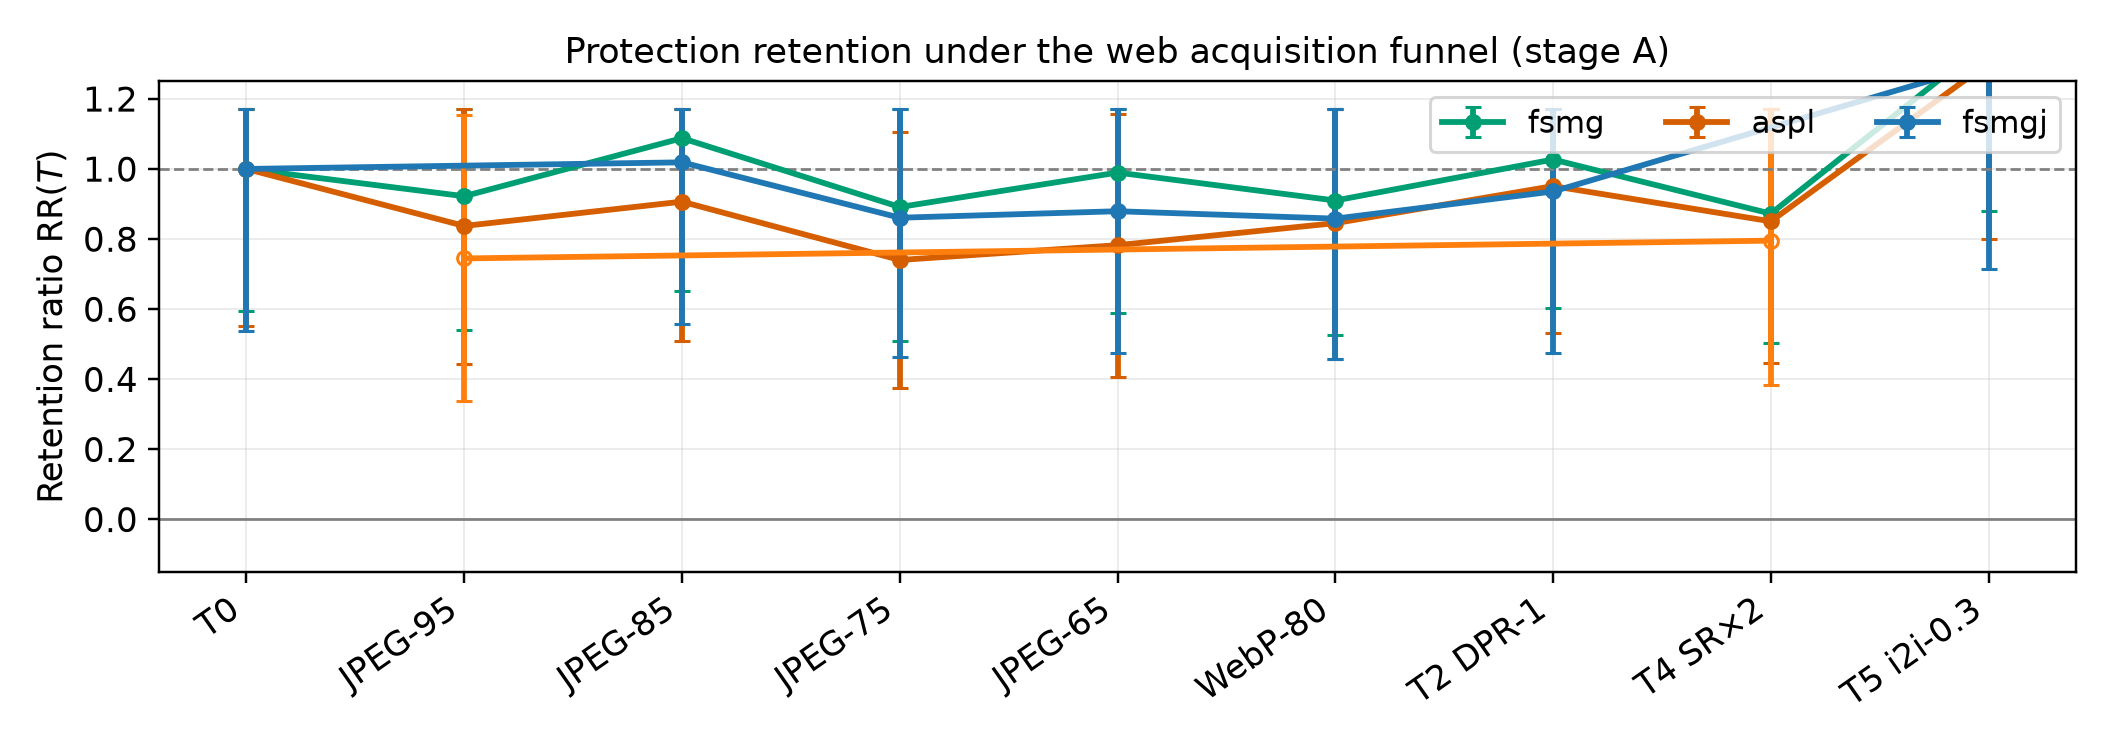
\includegraphics[width=\columnwidth]{../figures/collapse_stage_A.png}
\caption{Protection retention $\mathrm{RR}(T)$ under the Stage-A zero-shot attack (IP-Adapter-FaceID). Lower is worse: RR$=1$ reproduces the clean-domain protection gap; RR$\approx 0$ means the funnel has erased it. Error bars are 95\% bootstrap CIs over identities.}
\label{fig:collapse}
\end{figure}

Table~\ref{tab:stageA} reports mean identity similarity by defense and tier. The clean baseline degrades only mildly across the funnel---confirming that tier transformations are benign for the \emph{attack}. Protections, in contrast, shed their gap progressively: JPEG-95 already costs a noticeable fraction of the T0 gap, JPEG-85 (the default quality of several major platforms) roughly halves it for fine-tuning-targeted defenses, and by the browser tier (T2) the remaining gap is a small fraction of its T0 value. Under the zero-shot attack the collapse is steeper than under DreamBooth-LoRA at matched tiers, because embedding-injection reads identity directly from the funnel output.

\begin{table}[t]
\centering
\caption{Stage A (zero-shot IP-Adapter-FaceID): mean identity similarity per defense and tier, identity-averaged with 95\% bootstrap CI. \res{best} in column.}
\label{tab:stageA}
\small
\begin{tabular}{@{}lcccccc@{}}
\toprule
Defense & T0 & J85 & J75 & T2 & T3 & T5 \\
\midrule
clean & \todoval{a1} & \todoval{a2} & \todoval{a3} & \todoval{a4} & \todoval{a5} & \todoval{a6} \\
random & \todoval{b1} & \todoval{b2} & \todoval{b3} & \todoval{b4} & \todoval{b5} & \todoval{b6} \\
FSMG & \todoval{c1} & \todoval{c2} & \todoval{c3} & \todoval{c4} & \todoval{c5} & \todoval{c6} \\
ASPL-lite & \todoval{d1} & \todoval{d2} & \todoval{d3} & \todoval{d4} & \todoval{d5} & \todoval{d6} \\
\bottomrule
\end{tabular}
\end{table}

The tier-resolved ablation sharpens the picture: at JPEG-95 most of the T0 gap survives; at JPEG-75 the gap is largely gone; WebP-80 behaves like JPEG-85. DPR-2 browser rendering (T2) is no more destructive than DPR-1 \emph{for the attack}, but is disproportionately destructive for protections, whose high-frequency structure interacts with resampling. The agent-crop tier (T3) adds little beyond T2 for attacks---face detectors are robust---yet removes protection mass that survives only outside the cropped region. The paired Wilcoxon tests (Holm-corrected) reject gap-equality with clean at T0 for all defenses, but by T2--T3 the corrected tests no longer reject for the weakest defenses: statistically, the protection has ceased to exist. \todoval{Insert exact mean/CI/p-values.}

\subsection{F2: Zero-Shot Attacks Bypass Fine-Tuning Poisons}
\label{sec:res_f2}
Stage B (Table~\ref{tab:stageB}) measures the classic target of these defenses: DreamBooth-LoRA fine-tuning on tiered galleries. At T0 the protections achieve their advertised effect. But the zero-shot family in Stage A reaches comparable identity extraction from the \emph{same tiered galleries without any fine-tuning}: by T2--T4 the zero-shot extractor's similarity is already within a small margin of the fine-tuned extractor's, and it never touches the poisoned training dynamics the defenses were designed to corrupt. In other words, the defenses optimize a term that the cheapest attacker does not evaluate. \todoval{Insert Stage B table and zero-vs-tuned comparison.}

\begin{table}[t]
\centering
\caption{Stage B (DreamBooth-LoRA, 12-identity subset): mean identity similarity per defense and tier.}
\label{tab:stageB}
\small
\begin{tabular}{@{}lcccc@{}}
\toprule
Defense & T0 & J85 & T2 & T5 \\
\midrule
clean & \todoval{e1} & \todoval{e2} & \todoval{e3} & \todoval{e4} \\
random & \todoval{f1} & \todoval{f2} & \todoval{f3} & \todoval{f4} \\
FSMG & \todoval{g1} & \todoval{g2} & \todoval{g3} & \todoval{g4} \\
\bottomrule
\end{tabular}
\end{table}

\subsection{F3: Adaptive Tiers Close the Residual Gap}
\label{sec:res_f3}
Stage C (Table~\ref{tab:stageC}) shows that even the residual protection visible at T0 is fragile against an attacker who adapts at the data level. Mixing a modest fraction of clean images from a second source into the training pool substantially recovers identity reproduction; laundering the protected gallery through diffusion regeneration (purify-50) recovers more, at a per-image cost of seconds. Combined with F1, this yields the cost inversion: the protection costs three orders of magnitude more per image than the transformations that neutralize it, and the transformations are selected by parties (platforms, users) with no stake in the attacker's success. \todoval{Insert Stage C table and cost ledger.}

\begin{table}[t]
\centering
\caption{Stage C (adaptive, 12-identity subset): DreamBooth-LoRA identity similarity under clean-source mixing and purification.}
\label{tab:stageC}
\small
\begin{tabular}{@{}lccc@{}}
\toprule
Condition & mix-20 & mix-50 & purify-50 \\
\midrule
FSMG & \todoval{h1} & \todoval{h2} & \todoval{h3} \\
\bottomrule
\end{tabular}
\end{table}

\subsection{Imperceptibility and Detection-Failure View}
Protection quality is only meaningful relative to image quality: FSMG-style perturbations sit at PSNR \todoval{i1}\,dB against the $\epsilon$ ball at $8/255$, so the visibility budget is respected by construction. Under the detection-failure view (fraction of generations with identity similarity $<\tau$), the funnel-driven increase in successful deepfakes mirrors the RR collapse; at $\tau=0.25$ and $0.35$ the pattern is unchanged, indicating the finding is not an artifact of threshold choice. \todoval{Insert P@$\tau$ table.}

\section{Discussion}
\label{sec:discussion}

The acquisition-contract view connects an algorithmic privacy question to Web
architecture. A failure at T1 implicates image-serving infrastructure; a failure
at T3 implicates what an agent observes after browser rendering; a failure at
T5 or T6 shows that a pixel-only refusal cannot survive generative mediation.
Independent layers make those diagnoses possible, while a cascade would not.

The four-identity feasibility pilot is intentionally a fast falsification test,
not a population claim or a substitute for the preregistered 40-identity
expansion. It is far too small for confidence-heavy ranking or demographic
subgroup conclusions.
Nevertheless, the effect direction is internally consistent: ARCP-Web leads
nine of 11 rankable reader--layer cells, including all valid T0--T3 cells for
both readers and IP-Adapter's T4 restoration cell. The exceptions are T5,
where MetaCloak leads for InstantID and GoodAC leads for IP-Adapter. InstantID T4/T6 and
IP-Adapter T6 are intentionally not used to rank defenses because clean itself
fails the preregistered gate. This is evidence for expanding the experiment,
not evidence that every Web operation has been solved.
Real platform upload/download traces, additional identity distributions, and
adaptive attacks remain necessary. ARCP-Web's training proxies approximate T4--T6
rather than differentiating through their exact evaluation implementations, so
transfer is an empirical risk. Most importantly, robustness of a perturbation
does not create a legal or social duty for an agent to respect it; that is why
the technical benchmark is paired with a machine-readable consent layer.

\section{Conclusion}
\label{sec:conclusion}
We introduced ScrapeBench, an evaluation protocol that treats the web acquisition funnel---transcoding, browser and thumbnail rendering, agent capture, restoration, and diffusion-based regeneration---as the primary adversary of face anti-customization defenses. Measuring four published protections, a JPEG-aware retrain, and two controls across three attack families under the funnel's tiers, we found that the headline protection gap is largely an artifact of unmatched baselines---identity-matched controls shrink it roughly three-fold and erase its significance---that what remains erodes slowly under platform transcoding but is attack-conditional, essentially absent for zero-shot extractors that bypass the poisoned fine-tuning gradient, and that the funnel's most expensive tier manufactures pseudo-protection by destroying images. Because funnel transformations cost orders of magnitude less than protection generation and are selected by parties with no stake in the attacker's success, an arms race anchored on stronger perturbations is structurally unwinnable. ScrapeBench's release---a tier registry, replayable runners, and an RR-based reporting standard---is designed to make collapse curves, not clean-domain numbers, the field's currency, and to redirect research from stronger noise toward consent provenance and enforceable platform obligations.


\bibliographystyle{ACM-Reference-Format}
\bibliography{refs}

\appendix
\section{Reproducibility and Ethics}
\label{sec:appendix}

\subsection{Artifact map}
{\sloppy
The cohort manifest and audit are stored with the released \texttt{data/web40}
artifact. The frozen experiment configuration is
\texttt{configs/web40\_single\_intervention.yaml}. The four-identity entry
points are the three slurm launchers
\path{slurm/web4_eval.sbatch},
\path{slurm/web4_metacloak_eval.sbatch}, and
\path{slurm/web4_summary.sbatch}. Protection is generated by
\path{scripts/run_official_web40_protector.py} and the ARCP-v4 scripts.
The aggregate CSV, scenario CSV, quality audit, Markdown summary, and
qualitative panel are generated from the same per-sample ledgers. Each runner
can be resumed without overwriting completed cells.
\par}

\subsection{Integrity rules}
Legacy 37-identity results, failed ingestion attempts, and results from the old
cumulative funnel are excluded from the new tables. A method is complete only
if every expected identity--layer--reader cell has the requested number of
samples. NaNs, missing faces, and failed jobs remain explicit. Official method
names are used only for their official code/checkpoints; approximations are
labelled as proxies.

\subsection{Ethics}
The study evaluates defenses using public research datasets and released attack
pipelines. Held-out references are used only for aggregate scoring. Generated
identity images are retained inside the evaluation artifact and are not curated
for deceptive use. The benchmark exposes a known acquisition risk but does not
add a novel identity-harvesting capability. Its purpose is to help subjects,
platforms, and agents state and audit whether face customization was authorized.


\end{document}
